\documentclass[11pt]{article}
\usepackage{preamble}
\title{Two clocks: operator-level pressure--temperature decoupling measured across scales}
\author{Abdelrahman Saifelden\\ Alexandria Higher Institute of Engineering and Technology (AIET), Alexandria, Egypt\\ \texttt{Abdulrahman.Saifelden22011411@aiet.edu.eg}}
\date{\today}
\begin{document}
\maketitle

% ============================================================
\begin{abstract}
Pressure and temperature in a fluid are driven by the same source but evolve under
different operators: temperature obeys a local parabolic advection--diffusion
equation, while pressure in the incompressible limit obeys a global elliptic
constraint. We show that this operator split is measurable as distinct temporal and
spatial signatures across five independent settings. In field data, temperature
tracks the local diurnal cycle while pressure carries a planetary-scale semidiurnal
tide whose amplitude follows latitude, not local heating. In Rayleigh--B\'enard
direct numerical simulation, pressure and buoyancy share the same integral scale
but differ by a factor of 2.4 in Taylor microscale and $\sim 10^{4}$ in
high-wavenumber spectral power, with the gap widening as $Ra$ increases from
$10^{6}$ to $10^{8}$. In controlled compressible solvers, the hyperbolic-to-
elliptic crossover occurs on a timescale $t_{90} \approx 2.3\,L/c$, and the
fast-clock energy fraction scales as $M^{2}$. In the projection method, a single
elliptic solve reduces the divergence of the intermediate velocity field from
$2.7\times 10^{-2}$ to machine zero, while a spectrum-matched phase-randomized
surrogate leaves it unrepaired. Spectral equivalence is therefore not dynamical
equivalence: a field that matches an elliptic correction's power spectrum does
not reproduce its action as a constraint. In NCEP/NCAR reanalysis, the divergent
(fast) component of the wind carries $\leq 4\%$ of the kinetic energy, with a minimum at
the classical level of non-divergence. These measurements establish that the
two-operator structure is a robust, measurable property of real flows, with direct
implications for single-diffusivity turbulence closures.
\end{abstract}

% ============================================================
\section{Introduction}
\label{sec:intro}

A fluid heated from below or beside responds in its temperature field and in its
pressure field. These two responses are coupled through the equation of state and
the momentum balance, yet they are governed by different mathematical operators
with different Green's functions, different characteristic times, and different
spatial footprints. Temperature is transported: it is advected, diffused, and
filamented by the flow. Pressure, in the incompressible limit, is not transported
at all; it is the Lagrange multiplier of the divergence-free constraint,
determined instantaneously by a global elliptic solve. At finite compressibility,
that instantaneous adjustment is replaced by acoustic waves propagating at speed
$c$, but the adjustment remains fast compared to the advective timescale whenever
the Mach number is small.

This distinction is elementary at the level of the governing equations. Its
consequences for turbulence modeling, however, are rarely stated explicitly. The
standard closure assumption --- a single scalar eddy diffusivity acting on
resolved gradients, optionally with a fixed turbulent Prandtl number (Boussinesq
1877; Smagorinsky 1963) --- treats all transported quantities as if they respond
to stirring in the same way, on the same timescale, with the same spatial
structure. If pressure and temperature genuinely evolve under different operators,
this assumption is not merely approximate; it is structurally incomplete.

The purpose of this paper is to establish, quantitatively and across multiple
independent settings, that the operator split is measurable. We do not propose a
new closure; that is the subject of a companion paper (Saifelden 2026, hereafter
\textbf{P1}). We do not claim that single-diffusivity models are useless; we claim
that they are one-clock models applied to a two-clock system, and we measure the
discrepancy.

The paper proceeds as follows. Section~\ref{sec:operators} states the two-operator
structure and identifies the relevant timescales. Section~\ref{sec:temporal}
measures the temporal decoupling in atmospheric field data.
Section~\ref{sec:spatial} measures the spatial decoupling in direct numerical
simulation. Section~\ref{sec:demonstrations} demonstrates the mechanism in
controlled compressible and incompressible solvers. Section~\ref{sec:reanalysis}
confirms the energy split in the real atmospheric wind field.
Section~\ref{sec:discussion} discusses implications and limitations.

One result carries the paper's structural conclusion, so we preview it in
Fig.~\ref{fig:preview}: a phase-randomized surrogate that exactly matches the
power spectrum of the deterministic elliptic correction fails both pointwise and
as a constraint. The demonstration is developed in
Section~\ref{sec:projection}.

\begin{figure}[t]
\centering
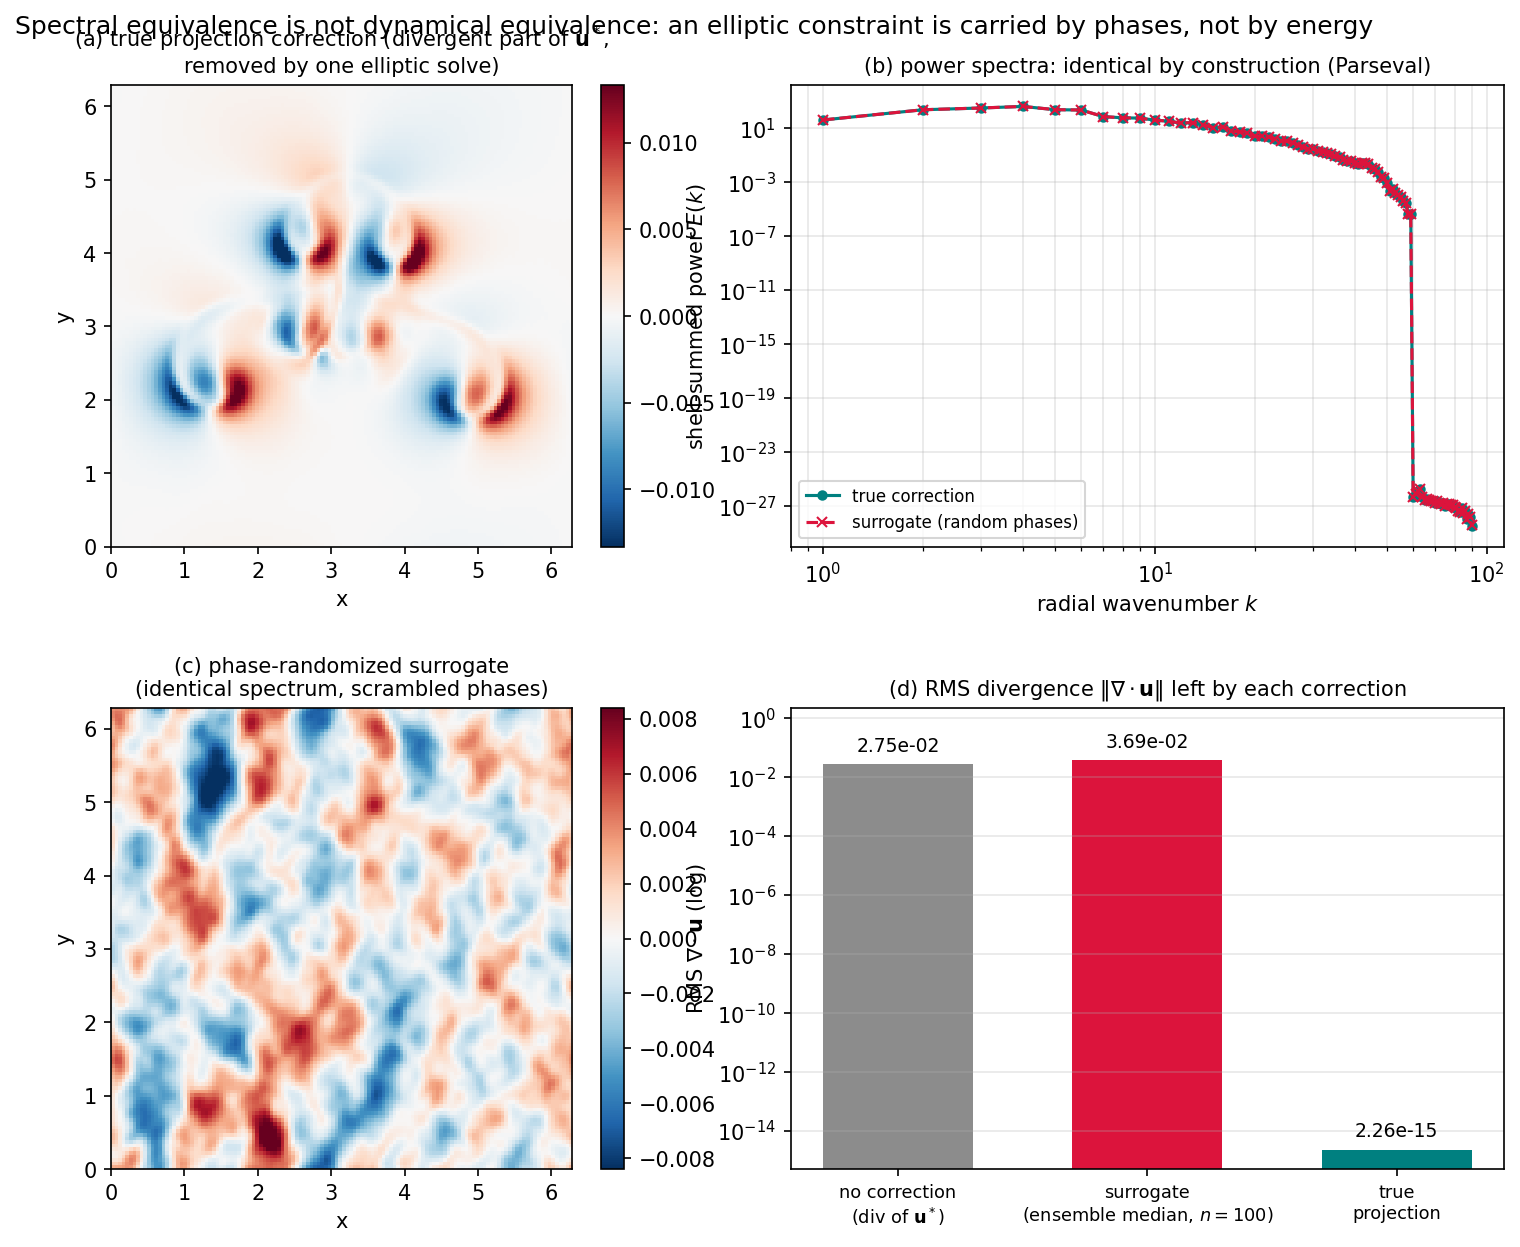
\includegraphics[width=0.82\linewidth]{figures/fig01_preview_surrogate.png}
\caption{Preview of the central demonstration, developed in
Section~\ref{sec:projection}. (a) The correction that one elliptic projection
removes from the slow, locally integrated drift $\mathbf{u}^*$. (b) Its power
spectrum and that of a phase-randomized surrogate: identical by construction
(Parseval-exact). (c) The surrogate field --- the same spectrum with scrambled
phases --- whose pointwise correlation with the true correction has ensemble
median $|r| = 0.07$ ($n = 100$). (d) RMS divergence of the velocity left by no
correction, by the surrogate, and by the true projection:
$2.7\times 10^{-2}$, $3.7\times 10^{-2}$, and $2\times 10^{-15}$,
respectively. Matching the energy content of an elliptic correction does not
reproduce its action as a constraint: spectral equivalence is not dynamical
equivalence.}
\label{fig:preview}
\end{figure}

% ============================================================
\section{The two operators}
\label{sec:operators}

\subsection{Governing equations}

Let $\mathbf{u}$ be velocity, $p$ pressure, $\theta$ a transported scalar
(temperature or buoyancy), and $\nu$, $\kappa$ the molecular viscosity and
diffusivity. The scalar obeys the parabolic advection--diffusion equation
\begin{equation}
\partial_t \theta + (\mathbf{u}\cdot\nabla)\theta
= \kappa\,\nabla^2\theta + S_\theta,
\label{eq:scalar}
\end{equation}
whose Green's function in the diffusive limit is a spreading Gaussian of width
$\sqrt{4\kappa t}$: local, causal, and memory-bearing.

In an incompressible flow, pressure is determined by the elliptic Poisson equation
obtained from the divergence of the momentum equation:
\begin{equation}
\nabla^2 p = -\rho\,\nabla\cdot\left[(\mathbf{u}\cdot\nabla)
\mathbf{u}\right] + \nabla\cdot\mathbf{f}.
\label{eq:poisson}
\end{equation}
Its Green's function is $\sim \ln r$ in two dimensions ($\sim -1/r$ in three
dimensions): global, instantaneous, and boundary-aware. In Fourier space,
$\hat{p} = -\hat{f}/k^2$; division by $k^2$ is a low-pass filter that suppresses
small-scale power by a factor $\sim 1/k^4$ relative to the source.

At finite compressibility, pressure instead satisfies the hyperbolic wave equation
\begin{equation}
\frac{1}{c^2}\,\partial_{tt}p - \nabla^2 p = s(\mathbf{x},t),
\label{eq:wave}
\end{equation}
with sound speed $c$. As $M = U/c \to 0$, Eq.~\eqref{eq:wave} degenerates into
Eq.~\eqref{eq:poisson}: the waves become infinitely fast and vanish into the
constraint (Klainerman \& Majda 1981).

\subsection{Timescales}

Three timescales are relevant for a domain of size $L$, flow speed $U$, and eddy
scale $\ell$:
\begin{equation}
\tau_p \sim \frac{L}{c}, \qquad
\tau_{\mathrm{adv}} \sim \frac{\ell}{U}, \qquad
\tau_\kappa \sim \frac{\ell^2}{\kappa}.
\label{eq:timescales}
\end{equation}
For air at laboratory-to-mesoscale $L$,
$\tau_p/\tau_{\mathrm{adv}} = M(L/\ell)^{-1} \ll 1$. Pressure equilibrates before
the flow moves; scalars integrate their history as the flow evolves. We refer to
the parabolic evolution of transported scalars as the \emph{slow clock} and the
elliptic/acoustic adjustment of pressure as the \emph{fast clock}. This
identification is an asymptotic statement rather than a metaphor: the slow clock
carries the scalar on the advective and diffusive timescales
$\tau_{\mathrm{adv}} \sim \ell/U$ and $\tau_\kappa$, while the fast clock
adjusts pressure on $\tau_p \sim L/c$. As $c \to \infty$ ($M \to 0$) the
fast-clock timescale vanishes and the hyperbolic wave equation degenerates into
the elliptic constraint of Eq.~\eqref{eq:poisson}: the fast clock stops
propagating and acts instantaneously, which is the limit in which the
measurements and simulations of this paper are taken.

% TODO (optional): schematic of the two operators (parabolic vs elliptic Green's
% functions and the three timescales of Eq.~\eqref{eq:timescales}). If created it
% would appear after Fig.~\ref{fig:preview}; none exists in the repository yet.
% \begin{figure}[t]
% \centering
% \includegraphics[width=0.85\linewidth]{figures/schematic_two_operators.png}
% \caption{Schematic of the two-operator structure. Left: the parabolic (slow)
% clock --- local, causal, memory-bearing, with a Gaussian Green's function.
% Right: the elliptic (fast) clock --- global, instantaneous, boundary-aware,
% with a $\ln r$ Green's function in 2-D. At finite compressibility the elliptic
% clock is replaced by a hyperbolic wave clock with speed $c$, which degenerates
% into the elliptic constraint as $M\to 0$.}
% \label{fig:schematic}
% \end{figure}

% ============================================================
\section{Temporal decoupling in field data}
\label{sec:temporal}

We first ask whether the two clocks are distinguishable in time-series
measurements at fixed locations. If pressure and temperature respond to the same
forcing on the same timescale, their spectra should be similar and their bulk
correlation should be tight. If they respond through different operators, their
spectra should differ qualitatively and their correlation should be weak and
regime-dependent.

\subsection{Single-site measurement: NEON eddy covariance}
\label{sec:neon}

We use the NEON bundled eddy-covariance product (DP4.00200.001) at the Wind River
Experimental Forest site (WREF; 45.82$^\circ$N, 121.95$^\circ$W; 53~m canopy
height) for January 2020 at 30-minute resolution: 1488 intervals, of which 1097
carry valid pressure and 1180 valid temperature (NEON 2020).

Figure~\ref{fig:neon} shows diurnal composites of incoming shortwave radiation,
air temperature, sensible heat flux, and barometric pressure. Three features are
apparent.

First, the source--response chain is causal and ordered: incoming shortwave leads
air temperature by approximately two hours and the sensible heat flux by
approximately three hours. The temperature signal is driven locally by solar
heating.

Second, the spectral characters of the two fields are qualitatively different.
Temperature variance is concentrated at the 24-hour diurnal line. Pressure
variance is dominated by multi-day synoptic variability with a distinct secondary
peak at the 12-hour semidiurnal atmospheric tide, visible as twin daily maxima in
the raw composite.

Third, the bulk daily correlation between pressure and temperature is weak:
$r(P,T) \approx +0.07$ ($R^2 \approx 0.005$). This is far from the tight positive
coupling that a constant-density ideal-gas relation would predict. The mismatch is
accommodated by density fluctuations of order one percent; the gas law holds
locally, but bulk pressure does not track bulk temperature.

\begin{figure}[t]
\centering

\includegraphics[width=0.86\linewidth]{figures/01_diurnal_composites.png}
\caption{NEON WREF, January 2020: diurnal composites of incoming shortwave
radiation, air temperature, sensible heat flux, and barometric pressure.
Temperature exhibits a single clean 24-hour signal driven by local solar heating.
Pressure shows a twin-peak semidiurnal tide superimposed on multi-day synoptic
variability.}
\label{fig:neon}
\end{figure}

A seasonal cross-check using July 2020 at the same site reproduces the qualitative
fingerprint at the opposite solar extreme. The temperature diurnal signal becomes
even cleaner (semidiurnal-to-diurnal power ratio drops from 7.3\% in winter to
1.0\% in summer), pressure retains its semidiurnal tide component, and the bulk
daily correlation shifts to $r = -0.49$ --- the summer thermal-low regime, in
which hot afternoons lower surface pressure. The sign and magnitude of the bulk
correlation are set by the synoptic regime; the spectral separation between the
two fields is not.

\subsection{Multi-station measurement: the latitude fingerprint of a global mode}
\label{sec:asos}

A single tower cannot distinguish ``pressure is noisy'' from ``pressure responds
to the whole atmosphere.'' To make this distinction, we examine one-minute
barometric and thermometric data from eight ASOS stations spanning
24.6$^\circ$--47.4$^\circ$N (Iowa Environmental Mesonet archive; Q1 2020).
Confidence intervals are computed via daily moving-block bootstrap ($n = 500$).

Table~\ref{tab:asos} summarizes the key measurements. The 24-hour temperature
amplitude varies with local insolation and surface type: it is largest at the
interior desert site (PHX, 5.06$^\circ$C) and smallest at the marine sites (SEA,
1.79$^\circ$C; EYW, 1.51$^\circ$C). It does not order monotonically with latitude.

The 12-hour pressure-tide amplitude, by contrast, decreases monotonically from
1.10~hPa at 24.6$^\circ$N to 0.34~hPa at 47.4$^\circ$N. This is the classical
signature of the global solar semidiurnal tide --- a planetary normal-mode
response whose amplitude is largest where the forcing projects onto the
low-latitude waveguide (Chapman \& Lindzen 1970). The trend correlation with the
migrating-tide climatology $A_H = 1.16\cos^3\varphi$~hPa (Haurwitz 1956) is 0.98.
Station totals fall in the range $0.9$--$1.4\times A_H$, consistent with the
expected contribution of non-migrating components (Dai \& Wang 1999).

\begin{table}[t]
\centering
\caption{Semidiurnal pressure-tide amplitude and diurnal temperature amplitude at
eight ASOS stations, Q1 2020. Bootstrap 95\% confidence intervals ($n=500$) are
given for the pressure-tide amplitude. The ratio to the Haurwitz migrating-tide
climatology $A_H = 1.16\cos^3\varphi$ is shown in the final column.}
\label{tab:asos}
\begin{tabular}{lcccc}
\toprule
Station & $\varphi$ & $S_{1,T}$ & $S_{2,P}$ [95\% CI] &
$S_{2,P}/A_H$ \\
 & ($^\circ$N) & ($^\circ$C) & (hPa) & \\
\midrule
EYW & 24.6 & 1.51 & 1.103 [1.013, 1.191] & 1.26 \\
MIA & 25.8 & 2.73 & 1.077 [0.979, 1.169] & 1.27 \\
MSY & 30.0 & 2.75 & 1.018 [0.878, 1.169] & 1.35 \\
DFW & 32.9 & 3.28 & 0.957 [0.794, 1.141] & 1.39 \\
PHX & 33.4 & 5.06 & 0.924 [0.861, 1.008] & 1.37 \\
DSM & 41.5 & 2.73 & 0.628 [0.398, 0.965] & 1.29 \\
CAR & 46.9 & 3.03 & 0.439 [0.181, 0.879] & 1.19 \\
SEA & 47.4 & 1.79 & 0.337 [0.262, 0.529] & 0.94 \\
\bottomrule
\end{tabular}
\end{table}

The interpretation is direct: pressure at a fixed site carries the signature of a
planetary-scale resonance, while temperature carries the signature of the local
solar cycle. The two fields share a forcing (the sun) but respond through
different operators with different spatial footprints. Station-level daily
pressure--temperature correlations range from $-0.05$ to $-0.56$, with bootstrap
95\% confidence intervals excluding any tight positive lock: the bulk coupling is
set by the synoptic regime, not by a gas-law link between the two fields.

Band-resolved coherence sharpens this statement. The magnitude-squared coherence
between hourly pressure and temperature is high (0.82--0.98) at the solar harmonic
lines, where both fields are phase-locked to the same astronomical forcing, and
above the phase-randomized surrogate 95\% level at all eight stations. In the
off-line sub-diurnal band (9--11~h and 13--20~h), coherence collapses to the
surrogate noise floor. Away from the shared solar clock, nothing locks the two
fields together (Fig.~\ref{fig:tide}).

\begin{figure}[t]
\centering

\includegraphics[width=0.95\linewidth]{figures/11b_tide_vs_latitude_ci.png}
\caption{Left: semidiurnal pressure-tide amplitude versus latitude at eight ASOS
stations with bootstrap 95\% confidence intervals, compared to the Haurwitz
migrating-tide climatology (dashed curve). The monotonic equator-to-pole decay is
the signature of a global resonance. Right: band-resolved coherence between hourly
pressure and temperature --- high at the shared solar lines, at the surrogate
noise floor off-line.}
\label{fig:tide}
\end{figure}

% ============================================================
\section{Spatial decoupling in direct numerical simulation}
\label{sec:spatial}

Field sensors measure time series at a point; they cannot resolve spatial
structure. A direct numerical simulation can. We use the two-dimensional
Rayleigh--B\'enard configuration from The Well dataset (Ohana et al.\ 2024):
$Ra = 10^6$, $Pr = 1$, $512\times 128$ grid, periodic in the horizontal, no-slip
walls, with velocity, buoyancy, and pressure co-resolved on the same grid.

\subsection{Same forcing, two geometries}

The central question is whether pressure and buoyancy, driven by the same
convective instability, develop the same spatial structure. The answer is no, and
the difference is precisely what the operator analysis of
Section~\ref{sec:operators} predicts.

At large scales, the two fields agree: both are organized by the convection rolls,
and their integral length scales are nearly identical (0.195 for buoyancy, 0.207
for pressure; ratio 1.06). At small scales, they diverge sharply. The Taylor
microscale of pressure is 2.40 times that of buoyancy, and the high-wavenumber
spectral power of buoyancy exceeds that of pressure by a factor of approximately
$10^4$ at $k \approx 10$.

Both numbers are direct consequences of the inverse Laplacian in
Eq.~\eqref{eq:poisson}. The factor $1/k^2$ in Fourier space suppresses pressure
power by $\sim 1/k^4$ relative to its source, so pressure remains smooth and
domain-spanning while buoyancy is advected into thin filaments with intense
small-scale gradients. Figure~\ref{fig:rb_fields} shows a snapshot;
Figure~\ref{fig:rb_spectra} shows the spectra.

\begin{figure}[t]
\centering

\includegraphics[width=0.86\linewidth]{figures/13_rb_fields.png}
\caption{Rayleigh--B\'enard DNS snapshot at $Ra = 10^6$: buoyancy (left) is
filamentary and sharp, organized into thin plumes; pressure (right) is smooth and
domain-spanning. Both fields are from the same simulation at the same instant.}
\label{fig:rb_fields}
\end{figure}

\begin{figure}[t]
\centering

\includegraphics[width=0.8\linewidth]{figures/15_rb_spectra.png}
\caption{Spatial spectra of buoyancy and pressure from the Rayleigh--B\'enard
DNS. The energy-containing scales coincide; at high wavenumber, buoyancy exceeds
pressure by $\sim 10^4$, consistent with the $1/k^4$ suppression of the inverse
Laplacian.}
\label{fig:rb_spectra}
\end{figure}

\subsection{Robustness across Rayleigh number}

The microscale ratio is not an artifact of a single Rayleigh number. Sweeping
$Ra = 10^6$, $10^7$, and $10^8$ using The Well's $Pr = 1$ test files (5
trajectories $\times$ 6 statistically steady snapshots each) yields the results in
Table~\ref{tab:ra_sweep}. The Taylor-microscale ratio grows from 2.58 at
$Ra = 10^6$ to 4.45 at $Ra = 10^8$, while the integral-scale ratio remains order
unity. As $Ra$ increases and buoyancy plumes sharpen toward finer scales, the
inverse Laplacian continues to hold pressure at the large scales. The operator
split widens with turbulence intensity rather than closing.

\begin{table}[t]
\centering
\caption{Taylor-microscale ratio ($\lambda_p/\lambda_\theta$) and integral-scale
ratio ($L_p/L_\theta$) as functions of $Ra$, from The Well $Pr=1$
Rayleigh--B\'enard dataset. Values are medians with 5--95\% ranges over 30
snapshots per $Ra$ (artifact \code{15b\_rb\_ra\_sweep.json}).}
\label{tab:ra_sweep}
\begin{tabular}{lcc}
\toprule
$Ra$ & $\lambda_p/\lambda_\theta$ & $L_p/L_\theta$ \\
\midrule
$10^6$ & 2.58 [1.98--3.59] & 1.02 [0.88--1.40] \\
$10^7$ & 2.94 [2.54--3.65] & 1.25 [1.03--1.85] \\
$10^8$ & 4.45 [3.27--5.88] & 1.75 [1.42--2.11] \\
\bottomrule
\end{tabular}
\end{table}

\subsection{Green's-function illustration}

To isolate the operator contrast from turbulence statistics, we apply a single
localized source to both the elliptic and parabolic operators in a developed
cavity flow. The elliptic response spreads over the entire domain: 79\% of its
magnitude lies beyond one source-width from the origin. The parabolic response at
matched time remains a confined Gaussian blob. Boundary geometry edits the global
pressure field instantly and only the local temperature field
(Fig.~\ref{fig:green}).

\begin{figure}[t]
\centering

\includegraphics[width=0.8\linewidth]{figures/39_elliptic_pressure.png}
\caption{Response to an identical localized source applied to both operators. The
elliptic (pressure) response spreads globally, with 79\% of its magnitude beyond
one source-width. The parabolic (heat-kernel) response remains confined.}
\label{fig:green}
\end{figure}

% ============================================================
\section{Dynamical demonstrations}
\label{sec:demonstrations}

The field data and DNS establish that the two-operator structure is measurable. We
now demonstrate the mechanism in controlled settings where every parameter is
known.

\subsection{The hyperbolic-to-elliptic crossover}
\label{sec:crossover}

A minimal two-dimensional linear-acoustics solver makes the relationship between
Eqs.~\eqref{eq:poisson} and \eqref{eq:wave} concrete. An initial pressure
perturbation radiates as a ring at speed $c$ and decays by geometric spreading.
Under sustained forcing, the compressible pressure relaxes to the same field as
the elliptic Poisson solve, with a final relative error of $\sim 2\times 10^{-3}$
for every sound speed tested.

The relaxation time scales as
\begin{equation}
t_{90} \approx 2.3\,\frac{L}{c},
\label{eq:t90}
\end{equation}
and the error histories for all sound speeds collapse onto a single curve when
time is rescaled as $ct/L$ (Fig.~\ref{fig:crossover}). The sound speed sets the
clock; the final state is independent of it. As $c \to \infty$, the adjustment
becomes instantaneous and the hyperbolic equation degenerates into the elliptic
constraint.

\begin{figure}[t]
\centering

\includegraphics[width=0.8\linewidth]{figures/17_crossover.png}
\caption{Relaxation of the compressible pressure field to the elliptic (Poisson)
solution for several sound speeds. All curves collapse in the rescaled time
$ct/L$, with $t_{90} \approx 2.3\,L/c$.}
\label{fig:crossover}
\end{figure}

\subsection{Both clocks in one nonlinear flow}
\label{sec:nonlinear}

A fully nonlinear two-dimensional isothermal compressible Navier--Stokes solver
(pseudo-spectral, periodic, with $p = c^2\rho$ so that $c$ is an explicit
parameter) is initialized from a Taylor--Green vortex at $Re \approx 600$. The
velocity field is Helmholtz-decomposed into solenoidal (vortical, slow) and
dilatational (acoustic, fast) components at each time step.

Table~\ref{tab:mach} summarizes the Mach-number sweep. The dilatational energy
fraction scales as $\sim M^2$, vanishing in the incompressible limit. The
time-averaged pressure (averaged over the fast acoustic period) converges to the
elliptic Poisson pressure with correlation approaching unity and residual shrinking
as $M^2$ (Fig.~\ref{fig:mach}).

\begin{table}[t]
\centering
\caption{Mach-number sweep in the nonlinear compressible solver.
$\langle KE_{\mathrm{dil}}\rangle / \langle KE_{\mathrm{sol}}\rangle$ is the
time-averaged ratio of dilatational to solenoidal kinetic energy. The pressure
residual is the RMS difference between the acoustic-averaged compressible pressure
and the elliptic Poisson pressure, normalized by the RMS pressure.}
\label{tab:mach}
\begin{tabular}{ccc}
\toprule
$M$ & $KE_{\mathrm{dil}}/KE_{\mathrm{sol}}$ &
Pressure residual \\
\midrule
0.05 & $1.5\times 10^{-4}$ & $8.1\times 10^{-4}$ \\
0.10 & $5.9\times 10^{-4}$ & $3.2\times 10^{-3}$ \\
0.20 & $2.3\times 10^{-3}$ & $1.4\times 10^{-2}$ \\
0.40 & $9.3\times 10^{-3}$ & $1.0\times 10^{-1}$ \\
\bottomrule
\end{tabular}
\end{table}

Two clocks coexist in one flow: the vortical energy decays on the slow advective
timescale while the acoustic energy oscillates on the fast period
(Fig.~\ref{fig:two_clocks}). Averaging over the fast clock acts as a low-pass
filter that recovers the elliptic limit --- an operation we will repeat on the
real atmosphere in Section~\ref{sec:reanalysis}.

\begin{figure}[t]
\centering

\includegraphics[width=0.82\linewidth]{figures/20_ns_two_clocks.png}
\caption{Nonlinear compressible box at $M = 0.1$: slow vortical energy decay with
fast acoustic oscillation superimposed. Both clocks are present in one flow.}
\label{fig:two_clocks}
\end{figure}

\begin{figure}[t]
\centering

\includegraphics[width=0.8\linewidth]{figures/21_ns_mach_sweep.png}
\caption{Mach-number sweep: dilatational energy fraction (circles) and
acoustic-averaged pressure residual (squares) both scale as $\sim M^2$ (dashed
line).}
\label{fig:mach}
\end{figure}

\subsection{The projection step as two-clocks synthesis}
\label{sec:projection}

The standard projection (fractional-step) method advances a Boussinesq flow by a
local drift followed by a global elliptic correction (Chorin 1968; Leray 1934):
\begin{align}
\mathbf{u}^* &= \mathbf{u}^n + \Delta t\left[
-(\mathbf{u}\cdot\nabla)\mathbf{u} + \nu\nabla^2\mathbf{u}
+ (b - \langle b\rangle)\hat{\mathbf{y}}\right],
\label{eq:drift}\\
\mathbf{u}^{n+1} &= \mathbb{P}\,\mathbf{u}^*,
\label{eq:project}\\
b^{n+1} &= b^n + \Delta t\left[
-(\mathbf{u}\cdot\nabla)b + \kappa\nabla^2 b\right],
\label{eq:scalar_step}
\end{align}
where $\mathbb{P} = I - \nabla(\nabla^2)^{-1}\nabla\cdot$ is the Leray projector.
The drift step (Eq.~\ref{eq:drift}) is a local, Markovian update --- the parabolic
clock. The projection step (Eq.~\ref{eq:project}) is a single global Poisson solve
--- the elliptic clock acting as a constraint.

Three results follow.

\emph{First}, the intermediate velocity $\mathbf{u}^*$ violates mass conservation
at RMS $\nabla\cdot\mathbf{u}^* \approx 2.7\times 10^{-2}$. A single projection
reduces this to $\approx 2\times 10^{-15}$ --- machine zero
(Fig.~\ref{fig:projection}).

\emph{Second}, replacing the projection correction by a phase-randomized field
with the identical power spectrum (Parseval-exact) --- the structural move of
spectrum-matched stochastic closures (Hasselmann 1976; Berner et al.\ 2017) ---
yields a pointwise correlation with the true correction of median $|r| = 0.07$
(95th percentile 0.20, over an ensemble of $n = 100$ surrogates). The RMS
divergence after the surrogate correction is $3.7\times 10^{-2}$
[$3.5$--$3.8\times 10^{-2}$, 95\% interval] --- no better than applying no
correction at all ($2.7\times 10^{-2}$; Fig.~\ref{fig:spde}).

\emph{Third}, the surrogate test establishes a general principle: spectral
equivalence is not dynamical equivalence. Two fields can share an identical
power spectrum and behave completely differently under a constrained operator,
because the elliptic correction acts through its phase geometry --- where fluid
must be moved --- not through how much energy it carries. The test targets the
specific hypothesis that matching the power spectrum of an unresolved correction
is sufficient to reproduce its constraint-preserving action; we do not claim that
all stochastic parameterizations fail, only that spectrum-matching alone does not
reconstruct a boundary-aware, globally coupled elliptic operator. The surrogate
test is performed in a two-dimensional periodic geometry; the structural
conclusion --- that randomization destroys the phase coherence through which the
elliptic operator enforces incompressibility --- holds in any domain in which the
constraint is imposed by a global Poisson solve, including bounded geometries
with nontrivial boundary conditions.

\begin{figure}[t]
\centering

\includegraphics[width=0.82\linewidth]{figures/23_projection_step.png}
\caption{One projection time step, dissected. Top: the divergent intermediate
velocity $\mathbf{u}^*$ (RMS $\nabla\cdot\mathbf{u}^* = 2.7\times 10^{-2}$).
Middle: the global elliptic potential $\phi$ satisfying $\nabla^2\phi =
\nabla\cdot\mathbf{u}^*$. Bottom: the projected, solenoidal velocity
$\mathbf{u}^{n+1}$ (RMS $\nabla\cdot\mathbf{u}^{n+1} = 2\times 10^{-15}$).}
\label{fig:projection}
\end{figure}

\begin{figure}[t]
\centering

\includegraphics[width=0.82\linewidth]{figures/24_spde_limit.png}
\caption{Spectrum-matched surrogate test. A phase-randomized field with the
identical power spectrum as the true projection correction (Parseval-exact) fails
to reproduce the correction pointwise: ensemble-median correlation $|r| = 0.07$
($n=100$), and the divergence constraint is left unrepaired (RMS
$\nabla\cdot\mathbf{u} = 3.7\times 10^{-2}$, compared to $2\times 10^{-15}$ for
the true projection).}
\label{fig:spde}
\end{figure}

% ============================================================
\section{The two clocks in the real atmospheric wind field}
\label{sec:reanalysis}

The preceding sections establish the operator split in controlled and
semi-controlled settings. We now ask whether the same structure is visible in the
real atmosphere.

\subsection{Method}

Horizontal winds from the NCEP/NCAR Reanalysis 1 (2.5$^\circ$ resolution; Kalnay
et al.\ 1996) are Helmholtz-decomposed on the sphere via spherical-harmonic
inversions $\nabla^2\psi = \zeta$ and $\nabla^2\chi = \delta$ into a rotational
(non-divergent, balanced) component and a divergent (fast) component. The same
decomposition is applied to the NCEP--DOE Reanalysis 2 (Kanamitsu et al.\ 2002) as
an independent cross-check.

Horizontal divergence is not a model artifact: by three-dimensional continuity, it
is the genuine footprint of vertical motion. The diagnostic is therefore the
energy split, not the existence of divergence.

\subsection{Results}

Table~\ref{tab:reanalysis} gives the ratio of divergent to rotational kinetic
energy at three pressure levels, from both reanalyses.

\begin{table}[t]
\centering
\caption{Ratio of divergent to rotational kinetic energy (daily mean) from
NCEP/NCAR Reanalysis 1 (R1) and NCEP--DOE Reanalysis 2 (R2). The minimum at
500~hPa corresponds to the classical level of non-divergence.}
\label{tab:reanalysis}
\begin{tabular}{lcc}
\toprule
Level & R1: $KE_{\mathrm{div}}/KE_{\mathrm{rot}}$ &
R2 cross-check \\
\midrule
850 hPa & 4.0\% & 4.5\% \\
500 hPa & 0.7\% & 0.8\% \\
250 hPa & 1.0\% & 1.1\% \\
\bottomrule
\end{tabular}
\end{table}

Four features emerge.

\emph{First}, the rotational wind dominates the kinetic energy at every level and
every resolved scale (Fig.~\ref{fig:reanalysis_wind}). Splitting by
spherical-harmonic degree $l$, the divergent branch sits one to two decades below
the rotational branch for all $l \leq 35$ (Fig.~\ref{fig:ke_spectrum}).

\emph{Second}, the vertical structure is physically meaningful: the divergent
fraction is smallest near 500~hPa --- the classical level of non-divergence
(Holton 2004) --- and larger in the boundary layer and near the jet outflow
(Fig.~\ref{fig:levels}).

\emph{Third}, the cross-check with Reanalysis 2 reproduces the same ordering and
the same 500-hPa minimum, with relative differences of 15\% or less. The ratio is
a property of the analyzed atmosphere, not of one assimilation system.

\emph{Fourth}, time-averaging acts as a low-pass filter on the fast clock: the
six-hourly ratio at 500~hPa (1.1\%) exceeds the daily-mean ratio (0.7\%).
Averaging scrubs the divergent component, exactly as acoustic averaging recovered
the elliptic pressure in Section~\ref{sec:nonlinear}.

\begin{figure}[t]
\centering

\includegraphics[width=0.86\linewidth]{figures/25_reanalysis_two_clocks.png}
\caption{NCEP/NCAR winds, one analysis day. Left: rotational wind (synoptic highs,
lows, and jets). Right: divergent wind (weak, confined to convergence and
overturning zones).}
\label{fig:reanalysis_wind}
\end{figure}

\begin{figure}[t]
\centering

\includegraphics[width=0.8\linewidth]{figures/26_reanalysis_ke_spectrum.png}
\caption{Kinetic-energy spectra by spherical-harmonic degree $l$: the divergent
branch sits one to two decades below the rotational branch at every resolved
scale.}
\label{fig:ke_spectrum}
\end{figure}

\begin{figure}[t]
\centering

\includegraphics[width=0.8\linewidth]{figures/27_reanalysis_levels.png}
\caption{Vertical structure of $KE_{\mathrm{div}}/KE_{\mathrm{rot}}$: minimum at
the level of non-divergence ($\sim$500~hPa). Six-hourly values (open symbols)
exceed daily-mean values (filled symbols), demonstrating that time-averaging acts
as a low-pass filter on the fast clock.}
\label{fig:levels}
\end{figure}

% ============================================================
\section{Discussion}
\label{sec:discussion}

\subsection{Summary of measurements}

The measurements, taken across the five settings examined in this paper ---
field observation, Rayleigh--B\'enard simulation, the controlled compressible
solvers, the projection method, and reanalysis --- consistently reveal the same
structure: pressure and temperature respond to the same forcing through different
operators with different timescales and different spatial footprints. The temporal
signatures differ (local diurnal versus planetary semidiurnal); the spatial
signatures differ (filamentary versus smooth, with a $1/k^4$ spectral gap); the
dynamical demonstrations show the mechanism (hyperbolic-to-elliptic crossover,
$M^2$ energy scaling, projection as synthesis); and the real atmosphere exhibits
the expected energy partition with the correct vertical structure.

\subsection{Implications for turbulence closure}

The measurements presented here have a direct implication for single-diffusivity
turbulence closures. A closure that models both momentum transport (shaped by the
global pressure field) and heat transport (shaped by local buoyant plumes) with a
single eddy diffusivity and a fixed turbulent Prandtl number assumes that the two
transport processes respond identically to changes in the shear-to-buoyancy ratio.
The field data show otherwise: binned by Monin--Obukhov stability (Monin \&
Obukhov 1954), the ratio of momentum to heat transport efficiency varies by a
factor of 4.3 in winter and 6.0 in summer at the NEON WREF site
(Table~\ref{tab:stability}). Stability-dependent variation of the individual
transport efficiencies is itself classical (Businger et al. 1971; Foken 2008;
Li 2019; Stull 1988); what is structural is that a single
fixed-Prandtl-number diffusivity cannot represent a 4--6$\times$ swing in their
ratio. This variation is consistent with the two-operator structure: momentum
transport is mediated by the global pressure field (fast clock), while heat
transport is mediated by local buoyant plumes (slow clock), and their relative
importance shifts with stability.

The spectrum-matched surrogate test of Section~\ref{sec:projection} further
constrains the class of admissible closure corrections: stochastic augmentations
that match the energy spectrum of the fast-clock correction but not its elliptic
geometry cannot repair the divergence constraint. The two failures are the same
failure: just as a single eddy diffusivity cannot represent the
stability-dependent split between momentum and heat transport
(Table~\ref{tab:stability}), a single spectrum cannot represent the
phase-dependent action of the elliptic split. A constructive closure that
addresses this limitation, building on optimal-prediction and Mori--Zwanzig
formulations of subgrid closure (Chorin, Hald, \& Kupferman 2000; Parish \&
Duraisamy 2017), is developed in the companion paper (Saifelden 2026).

\subsection{Scope and limitations}

All numerical demonstrations are two-dimensional and periodic. No
three-dimensional regularity claim is made. The reanalysis diagnostics are limited
to spherical-harmonic degree $l \leq 35$ and are based on model-assimilated
products, not raw observations. The field measurements span two months at the
seasonal extremes (NEON) and one season at eight sites (ASOS); they establish the
fingerprint of the operator split but do not constitute a global climatology.

\subsection{Reproducibility}

All figures and numerical results regenerate from the public repository at
\url{https://github.com/abdh0saifelden2-debug/K}. Each analysis is a single
command with fixed seeds, runnable on CPU. Input datasets are public: NEON
DP4.00200.001 (data.neonscience.org), ASOS one-minute data via the Iowa
Environmental Mesonet (mesonet.agron.iastate.edu), The Well Rayleigh--B\'enard
dataset (polymathic-ai), and NCEP/NCAR Reanalysis 1 via NOAA PSL OPeNDAP
(psl.noaa.gov). See Appendix~\ref{app:reproducibility} for the full command table.

% ============================================================
\section*{Acknowledgments}

The author thanks the National Ecological Observatory Network (NEON), the Iowa
Environmental Mesonet at Iowa State University, the Polymathic AI collaboration
for The Well dataset, and the NOAA Physical Sciences Laboratory for open access
to the data products used in this study, and the developers of the open-source
scientific Python ecosystem on which the analysis relies.

% ============================================================
\appendix

\section{Reproducibility}
\label{app:reproducibility}

Table~\ref{tab:stability} reports the Monin--Obukhov transport-efficiency
statistics behind the closure-relevant measurement of
Section~\ref{sec:discussion}, and Table~\ref{tab:commands} lists the commands
that regenerate each result in this paper.

\begin{table}[h]
\centering
\caption{Transport-efficiency statistics binned by Monin--Obukhov stability at
NEON WREF, January 2020 (602 usable 30-min periods). $r_{uw}$ and $r_{wT}$ are
the momentum and heat flux correlation coefficients (transport efficiencies);
the ratio is their median quotient. A July 2020 cross-check over 1{,}030 usable
periods shows the same ordering, with the ratio spanning 0.44--2.60 across the
classes --- a $\sim 6\times$ swing (artifact
\code{01b\_neon\_seasonal.json}).}
\label{tab:stability}
\begin{tabular}{lcccc}
\toprule
Stability class & $n$ & median $r_{uw}$ & median $|r_{wT}|$ & ratio \\
\midrule
strongly unstable & 95 & 0.182 & 0.209 & 0.87 \\
unstable & 73 & 0.324 & 0.150 & 2.17 \\
near-neutral & 121 & 0.312 & 0.095 & 3.28 \\
stable & 153 & 0.225 & 0.200 & 1.13 \\
strongly stable & 160 & 0.156 & 0.203 & 0.77 \\
\bottomrule
\end{tabular}
\end{table}

\begin{table}[h]
\centering
\caption{Reproducibility commands. All are runnable from the repository root with
fixed seeds and CPU-only execution.}
\label{tab:commands}
\small
\begin{tabular}{p{0.35\linewidth}p{0.55\linewidth}}
\toprule
Result & Command \\
\midrule
\S\ref{sec:neon} NEON diurnal composites &
\texttt{python general\_two\_clocks/run\_analysis.py} \\
\S\ref{sec:neon} Seasonal cross-check &
\texttt{python general\_two\_clocks/run\_neon\_compare.py} \\
\S\ref{sec:asos} ASOS latitude sweep &
\texttt{python general\_two\_clocks/asos/fetch\_iem.py \&\&
python general\_two\_clocks/run\_asos\_ci.py} \\
\S\ref{sec:spatial} RB DNS split &
\texttt{python general\_two\_clocks/run\_rb.py} \\
\S\ref{sec:spatial} $Ra$ sweep &
\texttt{python general\_two\_clocks/run\_rb\_ra\_sweep.py} \\
\S\ref{sec:spatial} Green's function &
\texttt{python general\_two\_clocks/run\_elliptic\_demo.py} \\
\S\ref{sec:discussion} Stability bins (Table~\ref{tab:stability}) &
\texttt{python general\_two\_clocks/run\_stability.py} \\
\S\ref{sec:crossover} Linear crossover &
\texttt{python general\_two\_clocks/run\_compressible.py} \\
\S\ref{sec:nonlinear} Nonlinear Mach sweep &
\texttt{python general\_two\_clocks/run\_compressible\_ns.py} \\
\S\ref{sec:projection} Projection / surrogate &
\texttt{python general\_two\_clocks/run\_boussinesq.py} \\
\S\ref{sec:reanalysis} Reanalysis split &
\texttt{python general\_two\_clocks/run\_reanalysis.py} \\
\bottomrule
\end{tabular}
\end{table}

% ============================================================
\section*{References}

Berner, J., et al. (2017). Stochastic parameterization: toward a new view of weather and climate models. \emph{Bulletin of the American Meteorological Society} 98, 565--588. doi:10.1175/BAMS-D-15-00268.1

Boussinesq, J. (1877). Essai sur la th\'eorie des eaux courantes. \emph{M\'emoires pr\'esent\'es par divers savants \`a l'Acad\'emie des Sciences} 23, 1--680.

Businger, J. A., Wyngaard, J. C., Izumi, Y., \& Bradley, E. F. (1971). Flux-profile relationships in the atmospheric surface layer. \emph{Journal of the Atmospheric Sciences} 28, 181--189.

Chapman, S., \& Lindzen, R. S. (1970). \emph{Atmospheric Tides: Thermal and Gravitational}. D. Reidel, Dordrecht.

Chorin, A. J. (1968). Numerical solution of the Navier--Stokes equations. \emph{Mathematics of Computation} 22, 745--762. doi:10.1090/S0025-5718-1968-0242392-2

Chorin, A. J., Hald, O. H., \& Kupferman, R. (2000). Optimal prediction and the Mori--Zwanzig representation of irreversible processes. \emph{Proceedings of the National Academy of Sciences} 97, 2968--2973. doi:10.1073/pnas.97.7.2968

Dai, A., \& Wang, J. (1999). Diurnal and semidiurnal tides in global surface pressure fields. \emph{Journal of the Atmospheric Sciences} 56, 3874--3902.

Foken, T. (2008). \emph{Micrometeorology}. Springer, Berlin.

Hasselmann, K. (1976). Stochastic climate models. Part I: Theory. \emph{Tellus} 28, 473--485. doi:10.1111/j.2153-3490.1976.tb00696.x

Haurwitz, B. (1956). The geographical distribution of the semidiurnal solar pressure oscillation. \emph{New York University Meteorological Papers} 2(5), 36 pp.

Holton, J. R. (2004). \emph{An Introduction to Dynamic Meteorology}, 4th ed. Elsevier Academic Press.

Kalnay, E., et al. (1996). The NCEP/NCAR 40-year reanalysis project. \emph{Bulletin of the American Meteorological Society} 77, 437--471.

Kanamitsu, M., Ebisuzaki, W., Woollen, J., Yang, S.-K., Hnilo, J. J., Fiorino, M., \& Potter, G. L. (2002). NCEP--DOE AMIP-II Reanalysis (R-2). \emph{Bulletin of the American Meteorological Society} 83, 1631--1643. doi:10.1175/BAMS-83-11-1631

Klainerman, S., \& Majda, A. (1981). Singular limits of quasilinear hyperbolic systems with large parameters and the incompressible limit of compressible fluids. \emph{Communications on Pure and Applied Mathematics} 34, 481--524. doi:10.1002/cpa.3160340405

Leray, J. (1934). Sur le mouvement d'un liquide visqueux emplissant l'espace. \emph{Acta Mathematica} 63, 193--248.

Li, D. (2019). Turbulent Prandtl number in the atmospheric boundary layer --- where are we now? \emph{Atmospheric Research} 216, 86--105. doi:10.1016/j.atmosres.2018.09.015

Monin, A. S., \& Obukhov, A. M. (1954). Basic laws of turbulent mixing in the surface layer of the atmosphere. \emph{Trudy Akademii Nauk SSSR Geofizicheskogo Instituta} 24, 163--187.

NEON (National Ecological Observatory Network) (2020). Bundled data products --- eddy covariance (DP4.00200.001), site WREF. https://data.neonscience.org

Ohana, R., et al. (2024). The Well: a large-scale collection of diverse physics simulations for machine learning. \emph{Advances in Neural Information Processing Systems (Datasets and Benchmarks Track)}.

Parish, E. J., \& Duraisamy, K. (2017). Non-Markovian closure models for large eddy simulations using the Mori--Zwanzig formalism. \emph{Physical Review Fluids} 2, 014604. doi:10.1103/PhysRevFluids.2.014604

Saifelden, A. (2026). What single-eddy-diffusivity closure discards: a Mori--Zwanzig audit, a scalar-independent memory time, and a divergence-cleaning design window. Companion manuscript, under editorial consideration at Physical Review (permanent submission ID assigned). \textbf{[P1]}

Smagorinsky, J. (1963). General circulation experiments with the primitive equations: I. The basic experiment. \emph{Monthly Weather Review} 91, 99--164.

Stull, R. B. (1988). \emph{An Introduction to Boundary Layer Meteorology}. Kluwer, Dordrecht.

\end{document}
